\newcommand{\todo}[1]{{\em \textcolor{red}{ #1}}}
\newcommand{\beq}{\begin{equation}}
\newcommand{\eeq}{\end{equation}}
\newcommand{\lang}{\langle}
\newcommand{\ra}{\rangle}
\newcommand{\vep}{\bm{\epsilon}}
\newcommand{\ep}{\epsilon}
\newcommand{\pars}{\vec{\theta}}
\newcommand{\dev}{\mathrm{d}}
\newcommand{\mstar}{h^{-1}M_\odot}
\newcommand{\hst}{\project{HST}}
\newcommand{\wfc}{\project{WFC3}}

\chapter{Super-resolution PSF model of HST WFC3-IR\chaplabel{wfc3ir}}

This \paper\ is joint work with Ross~Fadely (Insight) and David~W.~Hogg (NYU). 

\section{Chapter abstract}

Accurate model of the Point Spread Function is crucial for reliable point source photometry, astrometry, and weak lensing studies.
The PSF model of the $\hst$ $\wfc$ IR channel does not meet the accuracy required by these science goals. 
In addition, the PSF of the $\hst$ $\wfc$ IR 
channel is poorly sampled. Weak lensing studies of poorly resolved images of faint distant galaxies demands 
a great knowledge of the PSF sampled at a resolution higher than of the $\hst$ $\wfc$ pixels.

In this investigation, we present a generative model of every image taken by the $\wfc$ IR channel as a set of a number of point sources convolved
with the instrument PSF. In particular, we focus on modeling the pixel-convolved PSF, the instrument PSF convolved with the pixel response function. 

In particular, we model the images of point sources observed in the calibration program of the $\hst$ $\wfc$ IR channel in the \emph{F160W} bandpass. 
We expect the inference of the super-resolution PSF in the other bandpasses of the IR channel to follow a similar procedure. 
We discuss how the optimal solution of the problem can be found by using a variance model that correctly takes into account the model 
uncertainty and a regularization term that imposes a smoothness condition on the super-resolution PSF. 

\section{Introduction}

The Point Spread Function (hereafter PSF) determines the fraction of photons from a given point source that lands on a particular location 
from the center of that point source on a detector. The PSF of the $\hst$ $\wfc$ camera is extremely undersampled. That is, if a center of an observed star lies 
on the center of a pixel, a significant fraction of the brightness of that star will be 
encapsulated by the pixel that contains the centroid of the star.
In other words, within the full-width half-maximum (FWHM), the PSF is usually not spanned by multiple detector pixels since the designed 
pixels are large. This is mainly the result of a compromise made in design of the detectors to cover a wider field of view.

Poor sampling of the PSF by detectors renders many astronomical image processing tasks difficult. Precise astrometry and photometry 
of individual point sources requires knowledge of the PSF sampled on higher resolution than that of the detector pixels. 
In uncalibrated observations, the images of stars are generated by convolution of the point sources with the PSF and multiplication 
with a non-uniform detector sensitivity called the \emph{flat-field}. Flat-field corrections are important for photometry and astrometry of 
individual point sources. In under-sampled images, capturing the sub-pixel variations of the flat-field requires having a higher resolution 
model of the PSF. 

Furthermore, cosmic shear studies require accurate measurement of the shapes of individual distant galaxies. The galaxies used for estimation 
of the cosmic shear signal are faint and barely resolved by the $\hst$ $\wfc$ detectors. In order to reliably estimate the ellipticities of these poorly 
resolved galaxies, we need to convolve the model describing the light distribution of these galaxies with a higher resolution PSF model. 
Therefore, high resolution PSF is an essential ingredient in weak lensing studies of galaxies detected by the $\hst$ $\wfc$ IR 
channel.   

In this investigation, we focus on modeling the pixel-convolved PSF which is the optical (instrumental) PSF convolved with the 
pixel response function. It is the pixel-convolved PSF that can be directly estimated from observation without making any assumption 
about the sensitivity of detector pixels. Moreover, it is the pixel-convolved PSF that can be used to perform astrometry and photometry measurements as well as 
galaxy shape measurement for weak lensing analyses. All these procedures involve fitting a model to the pixel-convolved PSF. 

Alternatively, one can deliver a model of the optical (instrumental) PSF based on physical models of the telescope optics. 
This involves measurement of the optical wavefront at all locations across the focal plane and use of physically motivated parameters 
to model the image changes in wavefront. Significant progress has been made in exploring the space of physical models that can efficiently 
describe the optical PSF \citep{zernike,krist1995,krist2011,galsim_software}. 

Development of the optical models of the PSF are valuable efforts for simulations, validations, and understanding the systematic uncertainties 
that can affect astronomical inferences \citep{great3,galsim}. In practice however, using the optical PSF for photometry, astrometry and weak lensing studies 
requires fitting a star's model to the wavefront PSF model. The major drawbacks of this approach are the following: $(i)$ it does not make use of the observed 
data, and ${ii}$ it makes strong assumptions about sensitivity of detector pixels when it is used for model fitting. Since these reasons, we focus on building a 
data driven empirical model of the PSF. From now on in this \paper, we refer to the pixel-convolved PSF as the PSF. 

This \paper is structured as follows: In Section \ref{sec:data} we discuss the observations and data reduction. In Section \ref{sec:method} we discuss the algorithm we 
have developed for infering the super-resolution PSF model of the $\hst$ $\wfc$ IR channel observations. We present the preliminary results, and %FIXME
in Section{sec:summary} we summarize and conclude. 

\section{Data}\label{sec:data}

The $\wfc$ IR camera consists of four filters: F105W, F125W, F140W, F160W.
In what follows in the rest of this \paper\ we focus on modeling the images of point sources in the F160W filter of $\hst$ $\wfc$ IR channel. 
In our analysis, we make use of the FLT images that our calibrated with the recent models of charge transfer efficiency, flat-field, etc. 
We choose not use Drizzeled images \citep{drizzle,astrodrizzle} because they introduce correlated noise and 
distortions to the PSF that are not consistent across the image (a new algorithm \citep{olic} developed for the WFIRST mission does not suffer from these issues). 
This poses a challenge for optimal extraction of information and accurate measurement of shapes. Therefore the pixels in the FLT images are better-suited for performing PSF modeling. 

For each FLT image, we follow the following procedure to select stars with sufficiently high signal-to-noise ratio 
for PSF modeling. First the Source Extractor software \citep{sextractor} is run on each image to detect the objects. 
For each object, the stellarity index and blending/error flags are extracted. An object is called a \emph{star} if no blending/error flag is 
raised, its stellarity index is greater than 0.8 and if its peak pixel brightness values is 25 times greater than the median pixel brightness 
value.  

The FLT files obtained from the HST MAST archive are accompanied by Data Quality extension files. While extracting the super-resolution PSF model 
from the point sources in FLT images, pixels with data quality other than zero are not included in the model. This requirement guarantees that 
the damaged pixels do not contribute to the PSF model. For each point source, we extract a 25 pixels $\times$ 25 pixels patch that is centered on the brightest 
pixel of the point source.   

\section{Method}\label{sec:method}

\subsection{generative model}

We build our empirical model of the PSF by assuming that a given point source at the center of a patch can be described by 
the following quantities: 

\begin{itemize}
\item A global solution for the super-resolution PSF $X$ that is shared between all point sources across the field of view. We assume 
that $X$ is normalized to one and it is centered at the center of the central pixel of the patch. This super-resolution PSF is sampled on 
a grid with a higher resolution that the native pixel grid of $\hst$ $\wfc$ IR observations.

\item Centroid coordinate of a point source at a given patch $\Delta_n = (\Delta x_n, \Delta y_n)$. 
These two parameters dictate the offset between the position of the centroid of the point source $n$ with 
respect to the center of the patch.

\item Flux quantity $f_n$ which is the brightness of the point source.

\item A background quantity $b_n$ which sets the brightness level of the background sky.

\end{itemize}

Given these ingredients, we write down the generative forward model of the point sources in the center of patches in the following way:

\begin{eqnarray}
\mathbf{d}_{n} &=&  \mathbf{m}_{n} + \mathrm{noise}, \\
m_{n,i} &=& f_{n}K^{(n)}_{il} (\Delta_n) X_{l} + b_{n}. 
\label{eq:model}
\end{eqnarray} 

In Eq.~\ref{eq:model}, $\mathbf{d}_{n}$ is the observed 625 dimensional vector in patch $n$. $\mathbf{m}_{n}$ is the model of patch $n$ with the same dimensionality. The 
noise term \mathrm{noise} has a variance that we present shortly.
The operator $K^{(n)}(\Delta_n)$ is a linear operator that maps the super-resolution psf $X$ to a downsampled PSF at the native 
data grid. That is, when this operator is applied to $X$, it samples the $X$ on a downsampled grid (with the same resolution as the observations) 
that is shifted with respect to the grid on which $X$ is defined. The shift between the two grids is given by the vector $\Delta_n = (\Delta x_n , \Delta y_n)$.


We want to be able to explicitly construct these matrices so we can analytically compute the likelihood function and its derivative with respect to the super-resolution PSF $X$. 
We implement the linear sampling operator $K$ with bivariate cubic spline interpolation. We comparing our implementation of cubic-spline with that of the open source 
software $\mathtt{scipy}$ we note that they have consistent performances.

It is worth noting that there are many possibilities for designing the sampling operator $K$.  The simplest and fastest approach that one could 
choose is bilinear interpolation. But after applying this method to simulated PSFs, we find that this method lacks the sufficient accuracy we 
need for our forward model. Ideally, one could use a Sinc interpolation \citep{bickerton,galsim} which is an optimal choice for preserving information.
But we find sinc interpolation to be computationally very demanding for our purposes. Furthermore, we experimented with Gaussian Process interpolation for designing the downsampling matrix $K$. We found the Gaussian Process interpolation less advantageous than cubic-spline interpolation as it requires additional computing time for setting the hyper parameters of the kernel used in Gaussian Process.

\subsection{likelihood optimization}

Now that we have explained the quantities needed to quantify the generative model of $\wfc$ IR observations, we 
present our strategy for estimating the values of the parameters of individual point sources $\{f_{n},b_{n},\Delta_{n}\}_{n=1}^{N}$ and 
the global solution of the super-resolution PSF $X$.

The factor by which the PSF is undersampled varies from one filter to another. Our strategy for inferring the super-resolution of the PSF model of F160W filter is as follows. 
First we run the Source Extractor algorithm to identify all the stellar sources in the observed data. In this \paper\ we estimate $X$ on a 75 pixels $\times$ 75 pixels grid, which 
has a resolution three times that of the native pixel grid of the observations.

In order to estimate the PSF, we optimize the following likelihood function:

\begin{eqnarray}
-2 \ln L &=& -2 \sum_{n=1}^{N_{patches}} \ln L_{n} \label{eq:total} , \\
-2 \ln L_{n} &=& \sum_{i=1}^{N_{\rm pix}} \Big( \frac{\big(d_{n,i} - m_{n,i} \big)^{2}}{s^{2}_{n,i}} + \ln(2 \pi s_{n,i}^{2}) \Big) \label{eq:patch},
\end{eqnarray}
where $L_{n}$ is the likelihood of patch $n$, $L$ is the likelihood of the entire astronomical image, $s_{n,i}$ is the $i$th component of the 625 dimensional vector $\mathbf{s}_n$, and 
$\mathbf{s}_n^{2}$ is variance of the noise model in patch $n$. The variance is comprised of two terms, one arising from the Gaussian readout noise and another arising from the Poisson noise.
Therefore the total variance is given by a constant per-pixel variance of a Gaussian noise and a gain-like term that is proportional to the model $\mathbf{m}_{n}$:
\beq
\mathbf{s}_n^{2} = \sigma^{2} + g.\mathbf{m}_{n},
\eeq
where we extract Gaussian variance $\sigma^{2}=0.01$ and gain $g=0.05$ from the $\hst$ data. 

It is important to note that our forward model of the $\wfc$ IR 
observations given by euation ~\ref{eq:model} suffers from degeneracies. The first degeneracy is between 
the flux values $\{f_n\}$ and the super-resolution PSF $X$. This degeneracy will prevent us from finding a unique 
solution for $\{f_n\}$ and $X$. This degeneracy can be lifted by adding a reqularization term to Eq. \ref{eq:total} that imposes 
smoothness condition to $X$. 

We add the following term to the log-likelihood $L$
\beq
C_{\rm reg} &=& -2\ln L + \epsilon \sum_{j,k} \delta^{2}_{j,k},
\label{eq:reg}
\eeq
where the second term is the sum of the squared of the matrix $\delta$ whose $j,k$ components are given by the difference between the $j$th row and $k$th column of the super-resolution PSF 
and its nearest pixels. The prefactor $\epsilon$ sets the strength of the regularization term. This enforces our prior belief that the PSF should be a smoothly varying object.

The second type of degeneracy is the between the centroid offsets $\{\Delta_n\}$ and the super-resolution PSF $X$. In order to lift this degeneracy, we do not add any regularization 
term. Instead, throughout the optimization procedure we enforce a set of conditions that breaks will break this degeneracy. These conditions conditions enforce the super-resolution 
PSF to be normalized to one and centered around the central pixel of the higher resolution grid. 

For inference of the PSF, we follow an optimization procedure simillar to the wellknown method of Expectation Maximization. In the context of astronomy, this 
method has been employed in extreme deconvolution \citep{xd} and eteroscedastic matrix factorization \citep{hmf}. Finding the optimal solution of 
$X$ and $\{f_n , b_n , \Delta_n\}$ is done as follows. 

First we initialize the parameters $X$ and $\{f_n , b_n , \Delta_n\}$. We initialize the centroid offsets ${\Delta_n}$ by the matched-filter polynomial centroiding 
described in Chapter 1. In particular, we correlate a Gaussian kernel with FWHM of 2.0 pixels with the 5 $\times$ 5 central pixels of each patch before applying 
the polynomial centroiding method. The reason for why we apply the polynomial method to the central pixels of each patch is that many of the stars in our $\hst$ observations 
are in crowded fields and therefore applying the matched-filter centroiding method to the entire patch could lead to biases as a result of light contamination from overlapping 
or nearby sources. 

The initial background values $\{b_n\}$ are estimated by taking the median pixel value in each patch. For initializing the flux values $\{f_n\}$, first we subtract the initial 
estimates of background values from each patch. Afterwards, the $\{f_n\}$ values are initialized by computing the sum of the pixel values within 5$\times$5 apertures centered on 
the central pixels of the patches. The reason for limiting our initialization of the flux estimates to the 5$\times$5 apertures is to prevent light contamination of fluxes from 
overlapping and nearby sources. Besides since the PSF is poorly sampled, we expect the majority of the flux values to be captured by a few pixels in the centers of the patches. 

Lastly, the super-resolution PSF $X$ is initialized in the following way. First we subtract our intial estimates of the sky background levels from the pacthes. Then we divid the 
pixel values of the patches by their corresponding initial flux estimates. Then we use the cubic-spline interpolation method to interpolate the rescaled patches to a high resolution 
75 $\times$ 75 grid whose centers is shifted by $\{-\Delta_n\}$ with respect to the initial centroiding estimates. Afterwards, we evaluate the mean of the interpolated rescaled patches 
to get estimate the initial PSF. Furthermore, we normalize the PSF to one and interpolate it such that it is centered on the central pixel of the 75 $\times$ 75 high resolution grid.  

Now that we have initialzed the parameters of our model, we present the EM algorithm for optimizing them. At every iteration, we follow this 
iterative scheme. In the $n$th patch, we update $b_n$ by optimizing $L_n$ while holding $\{f_n, \Delta_n, X\}$ fixed. Then 
we update $f_n$ by optimizing $L_n$ while holding $\{b_n, \Delta_n, X\}$ fixed. Then we update $\Delta_n$ by holding $\{f_n, b_n, X\}$ fixed. 
Once $\Delta_n$ is updated, we update the sampling matrix $K^{(n)}$ accordingly. 

Once $\{b_n, f_n, \Delta_n\}$ for all patches, we update $X$ 
by optimizing the regularized cost function $C_{\rm reg}$ given in Eq.~\ref{eq:reg}. At every iteration, we normalize the super-resolution PSF and 
interpolate it such that it is centered on the center of the 75 $\times$ 75 grid. We repeat these iterations until the value of regularized cost function 
$C_{\rm reg}$ converges.

Note that we need to set the strength of the smoothness regularization term $\epsilon$. In order to so, we randomly divide the patches into to sets: 
the training set and the cross validation set. We select a set of values $S_{\epsilon} = \{0.01,0.1,1,10,100\}$ for the parameter $\epsilon$. We then modify the optimization 
procedure as follows. First, we select a value of $\epsilon$ from $S_{\epsilon}$. Then given the selected $\epsilon$ we follow the optimization procedure as described above to 
the patches in the training sample to estimate $X$ as well as the parameters $\{f_n,b_n,\Delta_n\}$. 

Once $X_{\epsilon}$ is estimated assuming a value for the parameter $\epsilon$, we optimize the patch negative log-likelihood $-2\ln L_n$ given in Eq.~\ref{eq:patch} to find a solution for $\{f_n,b_n,\Delta_n\}$
variables for every patch in the cross validation set. We then sum up the optimal values of $-2\ln L_n$ in the cross validation patches to compute the cross validation score $C_{\rm cv}$ as a function of 
regularization strength $\epsilon$

\beq
C_{\rm cv} (\epsilon) = -2 \sum_{n} \ln L_{n}^{\star} \; \mathrm{where} \; L_{n}^{\star} = \mathrm{max} \{ L_{n}(X_{\epsilon})\}
\eeq

In the end, we select the super-resolution PSF $X_{\epsilon}$ that minimizes the cross-validation cost function $C_{\rm cv} (\epsilon)$.

%We follow something like \citep{xd,hmf} heteroscedastic matrix factorization ....
%Simillar methods in the literature that rely on compressed sensing \citep{ngole,ngole2}

Sofar we have not addressed the problem of how our generative forward model of the patches takes into account the light contamination arising from 
the overlapping or nearby sources. Ideally one would use the bright isolated sources to estimate the PSF. This issue is particularly alarming since 
a considerable number of point sources in our collected $\wfc$ IR observations are present in crowded regions. 

In order to alleviate the issue arising from the light contamination of patches, we modify the noise model by introducing an additional term to the variance 
of the noise. This additional term is proportional to squared downsampled model of the patch. This accounts for the discrepancy between the downsampled PSF model of the 
point source at the center of the patch and the observed patch. The modified variance model is given by
\beq
\mathbf{s}_n^2 = \sigma^{2} + g\mathbf{m}_{n} + q\mathbf{m}_{n}^{2},
\label{eq:modified_variance}
\eeq 
where in principle, the dimensionless parameter $q$ is large when we have do not have a good knowledge of the PSF model and should become 
smaller as our knowledge of the PSF improves. 

Furthermore, we use a $\chi^2$ clipping technique to clip ill-fit portions of the patches. 
This clipping step will prevent the light contamination by overlapping sources to bias the infered parameters. 
At every iteration of optimizing the log-likelihood function, we mask out the pixels for which the clipped $\chi^{2}$ 
(denoted by $\chi^{2}_{clip}$ from now on) is larger than 3. For a given patch $n$, the clipped $\chi^{2}$ is defined in the folowing way:
\beq
\chi^{2}_{n,\mathrm{clip}} &=& \frac{(\mathbf{d}_{n} - \mathbf{m}_{n})^{2}}{\mathbf{s}_{n}^{2}}, 
\eeq
where $\mathbf{s}_{n}^{2}$ is given Eq.~\ref{eq:modified_variance}. In a given patch $n$, the log-likelihood pixels with $\chi^{2}_{n,\mathrm{clip}} > 3$ 
do not contribute to computation of $L_n$ and its derivatives with respect to model variables. 
We set the parameter $q$ to 1. We note that this choice of does a good job at masking out the pixels that recieve light from the nearby or overlapping sources. 
In principle $q$ needs to decrease iteratively as our knowledge of the PSF improves. In this work however, we choose to hold the value of $q$ fixed at one. 

The algorithm we use for inference of the super-resolution PSF $X$ is summarized in Algorithm ~\ref{alg:supermean}.

\begin{algorithm} 
\caption{The procedure for Inferring the Super-Resolution PSF}
\begin{algorithmic}[1] \label{alg:supermean}

\IF{$t=1:$}
\STATE $\epsilon_t \gets \infty$
\FOR{$n=1,...,N$}
   \STATE // \emph{This can now be done in parallel for all i}

   \STATE $b_{n}$ \gets \mathrm{median} \; $(y_{n})$
   \STATE $f_{n}$ \gets $\sum_{i=1}^{N_pix} \big(y_{n,i} - b_{n}\big)$
   \STATE \mathrm{Initialize} $\Delta_{n}$ with the 3 \times 3 polynomial method
   \STATE $X_{n}$ \gets \mathrm{cubic \; spline} $(\Delta_n)[\big(y_{n,i} - b_{n}\big)/f_n]$
\ENDFOR
\STATE $X$ \gets $\sum_{n=1}^{N} X_{n]$

\ENDIF
\IF{$t=2,...,N_{it}:$}
\FOR{$i=1,...,N$}

   \WHILE{$\rho(X,D)>\epsilon_t$}
   \STATE Draw $\pars^{*}_{t}$ from $\{\pars_{t-1}\}$ with probabilities $\{w_{t-1}\}$
   \STATE $\pars^{*}_{t} \gets K(\pars^{*}_{t},.)$
   \STATE $X = f(\pars^{*}_{t})$
   \ENDWHILE
   \STATE $\pars^{(i)}_{t} \gets \pars^{*}_{t}$
   \STATE $w^{(i)}_{t} \gets \pi(\pars^{(i)}_{t}) / \big(\sum\limits_{j=1}^{N}w_{t-1}^{(i)}K(\pars^{(j)}_{t-1},\pars^{(i)}_{t}) \big)$
\ENDFOR
\ENDIF

\end{algorithmic}
\end{algorithm}

\section{Preliminary Results}\label{sec:results}

With the ingredients of our methodology explained in Section~\ref{sec:method}, we now present the results of applying our 
method to the observations of the point sources in $\hst$ $\wfc$ IR channel. First, we train our PSF model with a number of 
patches that were selected such that majority of them only contain one point source. 

In principle given the methodology explained in Section~\ref{sec:method}, we can train our model forward model on patches with arbitrary 
number of stars. But in order to minimize the training time as much as possible, we follow this selection criteria for the training sample.
It is important to note that selecting single-point source patches does not necessarily guarantee no light contamination by the nearby sources, 
especially by bright objects in nearby patches.

Therefore it is necessary to follow the procedure explained in the previous section to clip the pixels that may have received light 
contamination from the nearby sources. The parameter $q$ will be held at the constant value of one and any pixel with $\chi^{2}_{\rm clip} > 3 $ 
will not be permitted to contribute to the likelihood function. 
This will ensure ill-fit portions of the training pixels will not bias the final PSF estimate. 

In what follows in the remainder of this \paper\, we set the the strength of the smoothness regularization $\epsilon$ to 10$^{3}$ and hold 
it fixed. Although it is important to set the value of $\epsilon$ by minimizing a cross-validation score, in practice one can choose a 
value for $\epsilon$ by ensuring that neither the negative log-likelihood nor the regularization term will dominate each other. 

Choosing an arbitrarily large value of $\epsilon$ will drive the optimization procedure to maximize smoothness, while choosing a very small 
value of $\epsilon$ will make the smoothness regularization negligible. We found that with $\epsilon = 1000$, the contributions received from the 
right hand sides of Eq.~(\ref{eq:reg}) remain similar. We will make use of the cross-validation set for validating our estimate of the 
super-resolution PSF and our methodology for masking the contribution of nearby stellar sources to patch fitting.  

In Figure~\ref{fig:srpsf} we show our initialization of the super-resolution PSF method and our final estimate of the PSF found form 
minimizing Eq.~(\ref{eq:reg}). We note that in comparison to the final estimate of the PSF, our initaial estimate based on scaling, shifting, 
upsampling and averaging is very smooth. The initial PSF misses many of the sharp features along the tails of the final estimate. Furthermore, 
it appears to have a peak with less sharpness toward the center.

 


\section{Discussion}\label{sec:summary}

In this work, we have presented the first generative forward model of the observations of point sources in $\hst$ $\wfc$ IR 
observations. The PSF of $\wfc$ IR channels are the most undersampled amongst all $\hst$ channels. 
The exersize of making highly accurate masurements of the shapes of faint poorly resolved galaxies, accurate and precise astrometry and photometry of point sources, 
correction of the variable sub-pixel response function ``flat-field'' of the telescope, and many other scientific applications require excuisitely accurate model of 
the PSF at a resolution higher than what can be sampled by the $\wfc$ IR detectors. 

Our approach differs from the analysis presented in \citet{ngole,ngole2} in that it does not any infer the super-resolution PSF in a wavelet basis and it does not 
imposes any sparsity regularization. Our analysis is different than the approach of \citet{anderson2000} as we estimate the PSF by optimizing a well-motivated objective function 
that is based on a generative forward model of the observations. 

The method presented in \citet{anderson2000} is based on shifting, averaging and eventually smoothing the PSF.
Furthermore, it is restricted to using only the isolated point sources and it is not prone to patches in which there is light contamination by the nearby sources. 
The method presented in this \paper\ implements a rigorous treatment of overlapping sources by modifying the variance of the noise model. 



%%%%%%%%%%%%%%%%%%%% FIGURES %%%%%%%%%%%%%%%%%%

%%%%%%%%%%%%%%%%%%%%%%%%%%%%%%%%%%%%%%%%%%%%%%%%%%%%%%%%
% PSF INITIAL AND FINAL
%%%%%%%%%%%%%%%%%%%%%%%%%%%%%%%%%%%%%%%%%%%%%%%%%%%%%%%%

\begin{figure*}
 \begin{tabular}{cc}
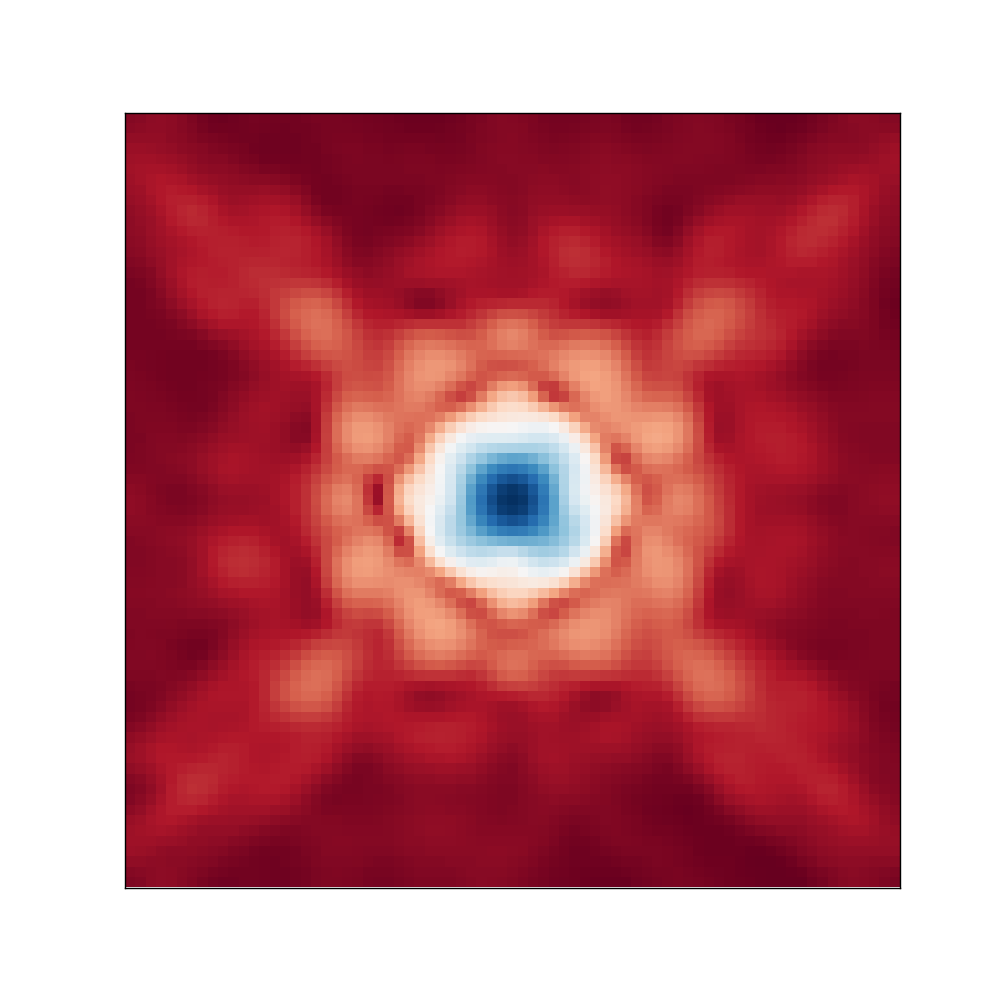
\includegraphics[width=0.5\textwidth]{figures/wfc3ir/super0.png}
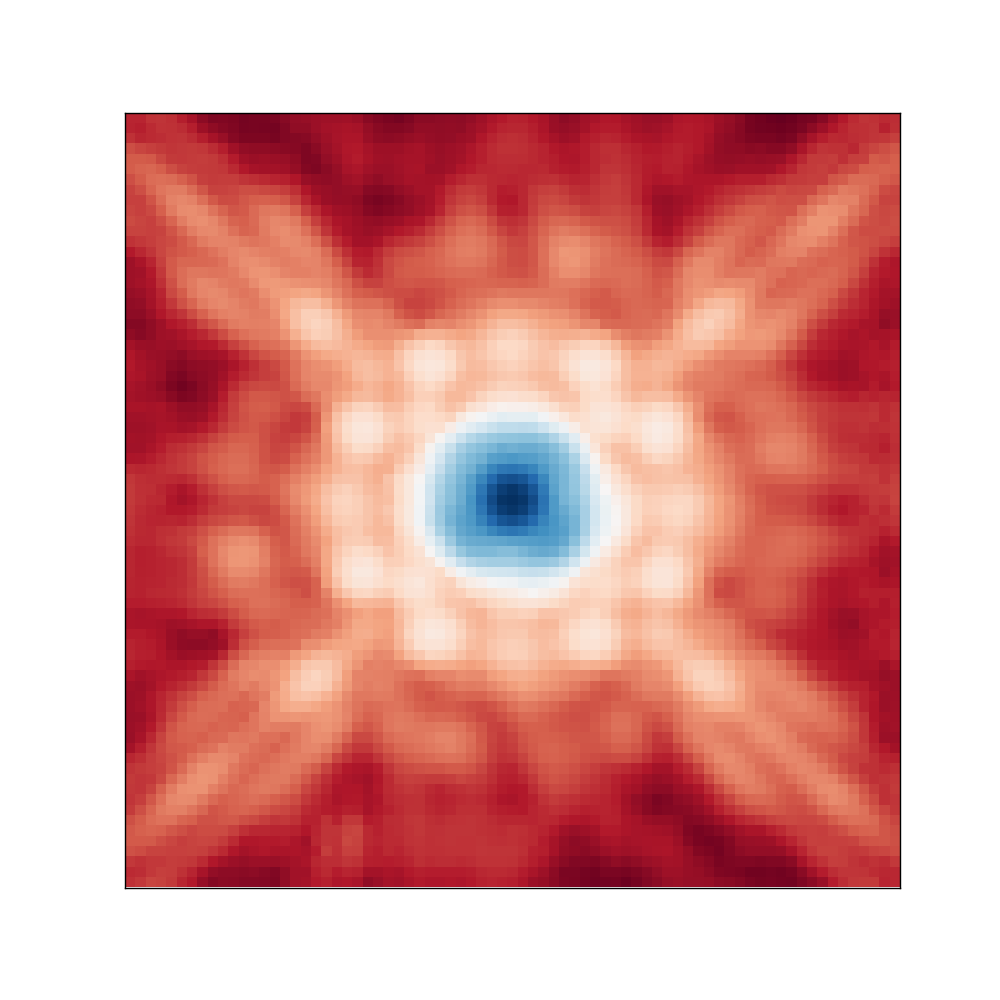
\includegraphics[width=0.5\textwidth]{figures/wfc3ir/super2.png}
\end{tabular}
\caption{\label{fig:srpsf} Left: Demonstration of the initialization of the super-resolution PSF model. The initial PSF was constructed by scaling (background subtraction and flux normalization), shifting (through matched-filter polynomial centroiding), upsampling (with cubic spline interpolation), and averaging the isolated stars in the observation sample. 
Left: Demonstration of the super-resolution PSF estimate after optimizing the likelihood function with six iterations. Note how the averaged upsampled initial PSF is smooth and lacks the sharp features visible at tails of the optimized super-resolution PSF.}
\end{figure*}

\begin{figure*}
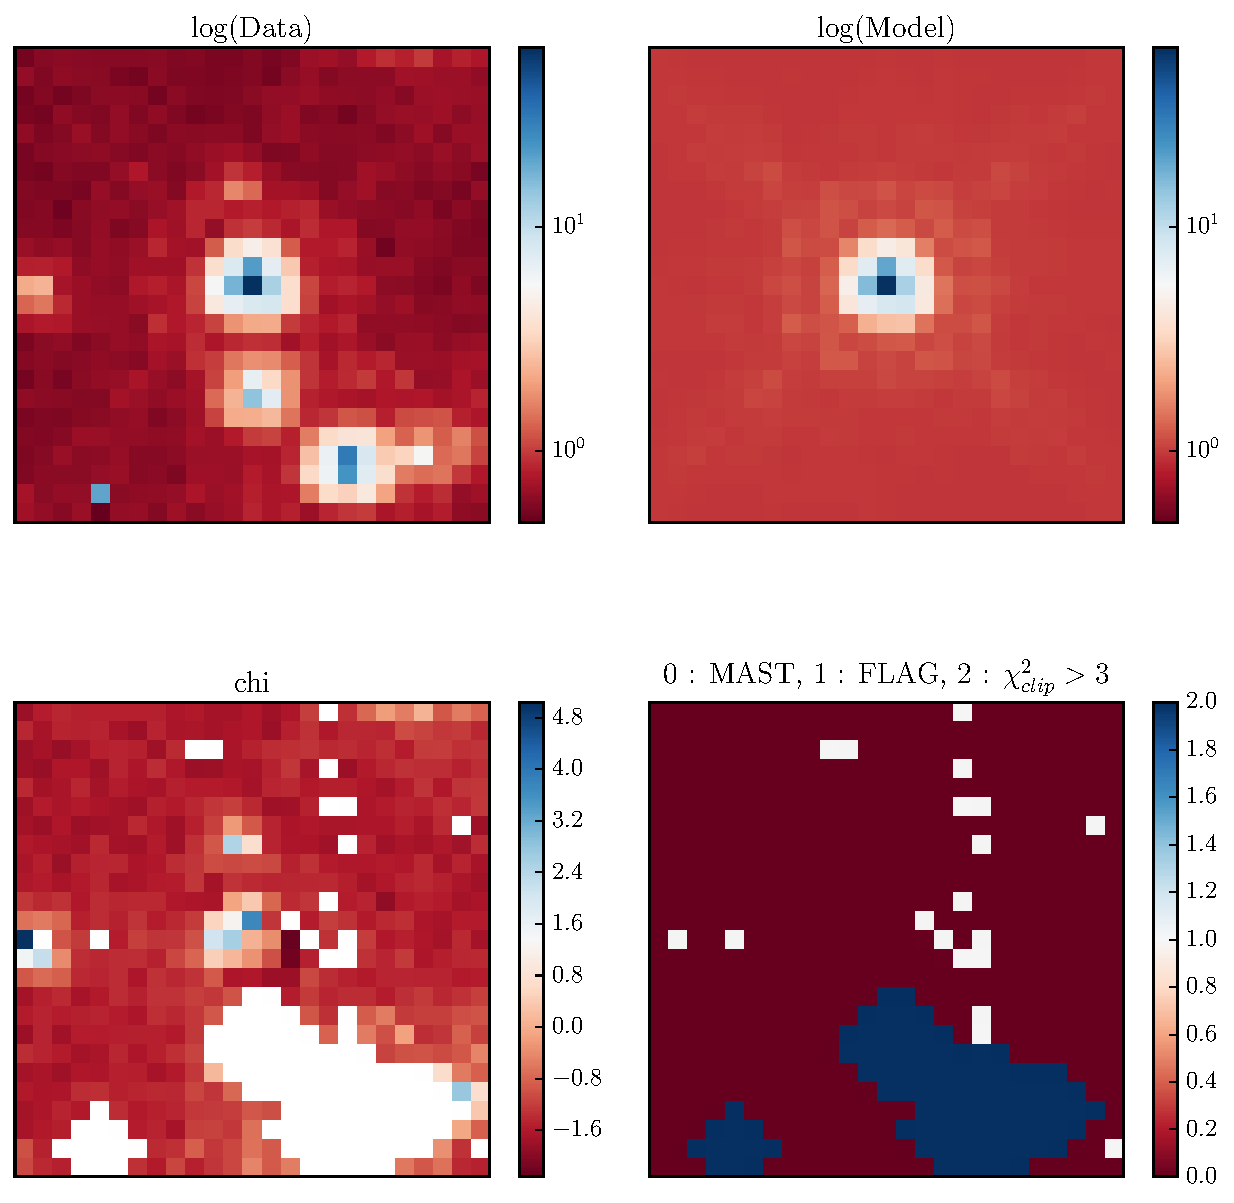
\includegraphics[width=0.9\textwidth , height=0.9\textwidth ]{figures/wfc3ir/example1762.pdf}
\caption{\label{fig:validation_1} }
\end{figure*}

\begin{figure*}
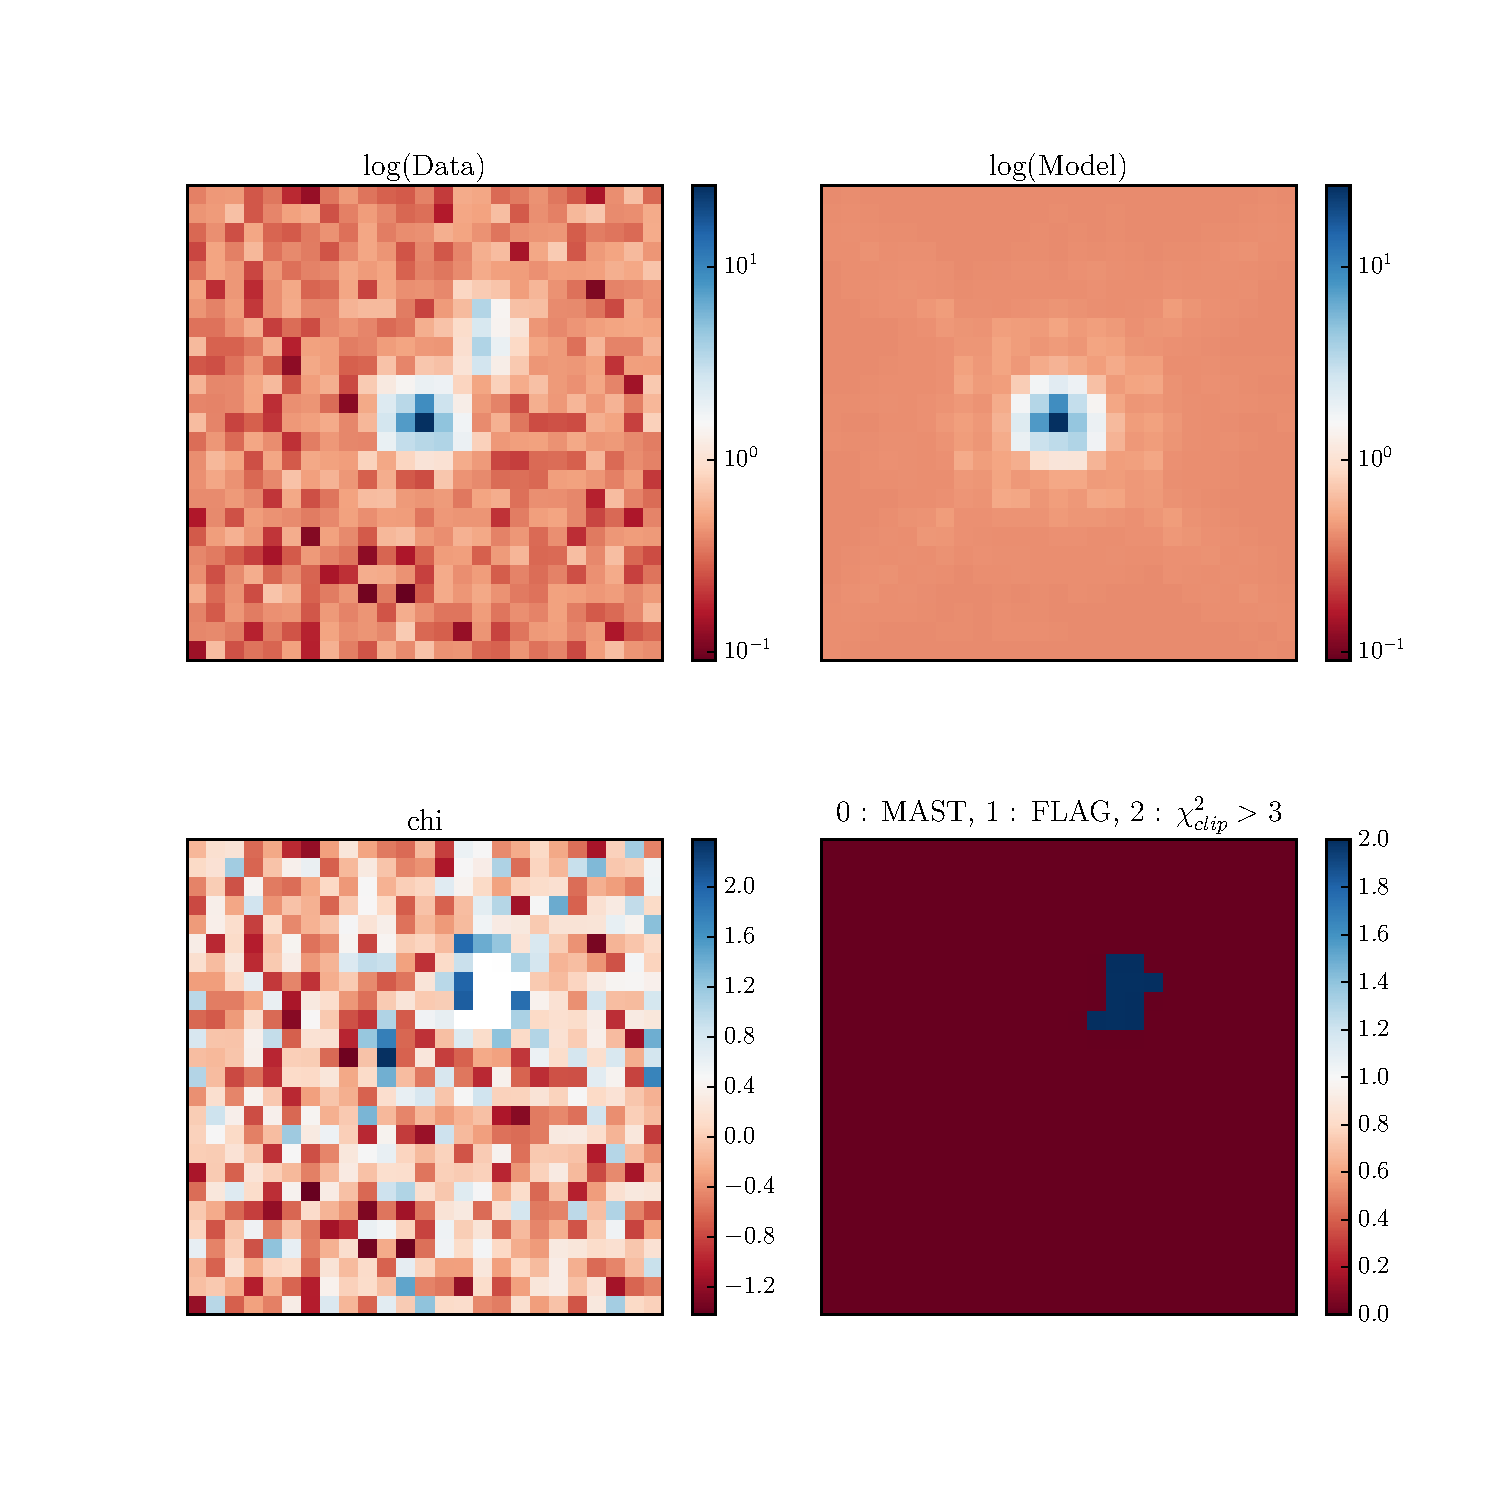
\includegraphics[width=0.9\textwidth]{figures/wfc3ir/example7.pdf}
\caption{\label{fig:validation_2} }
\end{figure*}

\begin{figure*}
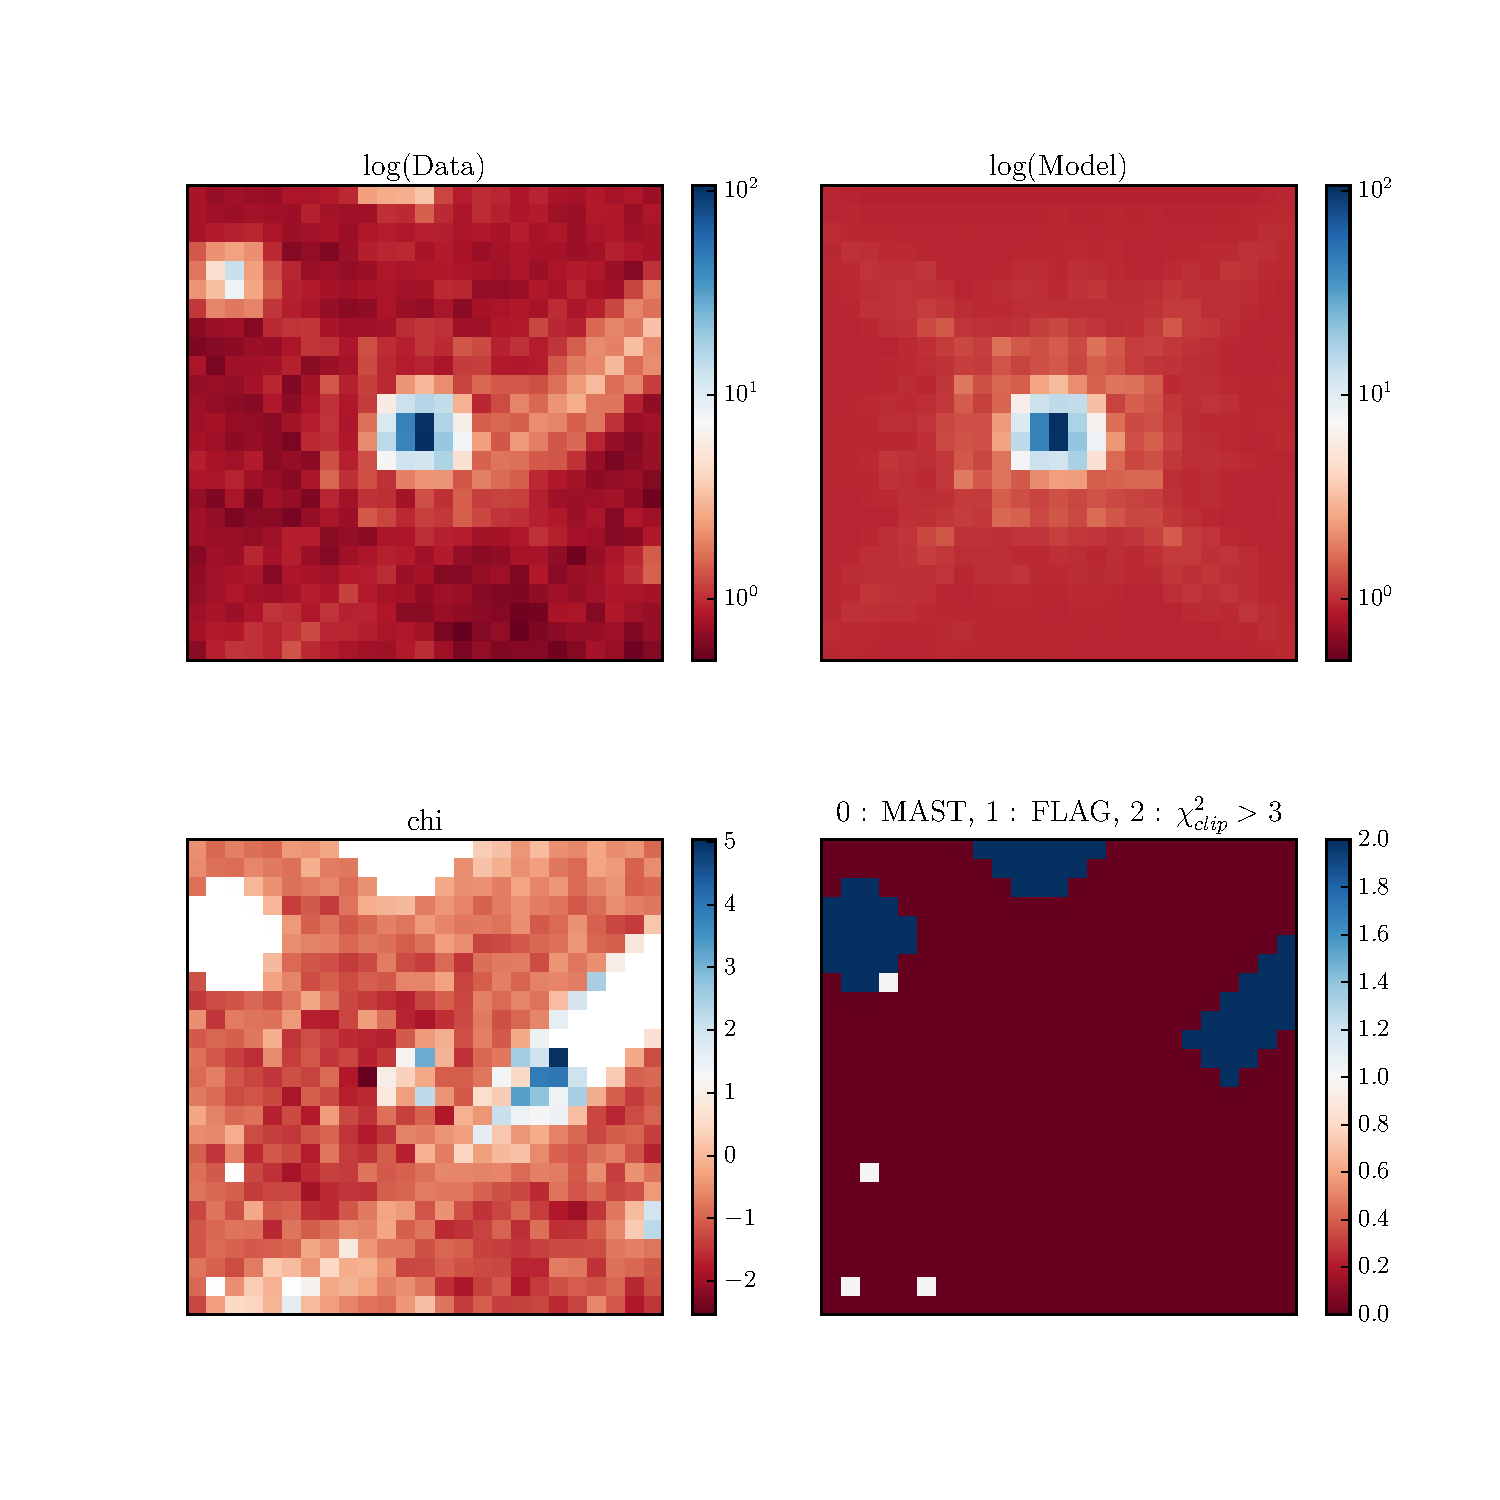
\includegraphics[width=0.9\textwidth]{figures/wfc3ir/example11.pdf}
\caption{\label{fig:validation_3} }
\end{figure*}


\begin{figure*}
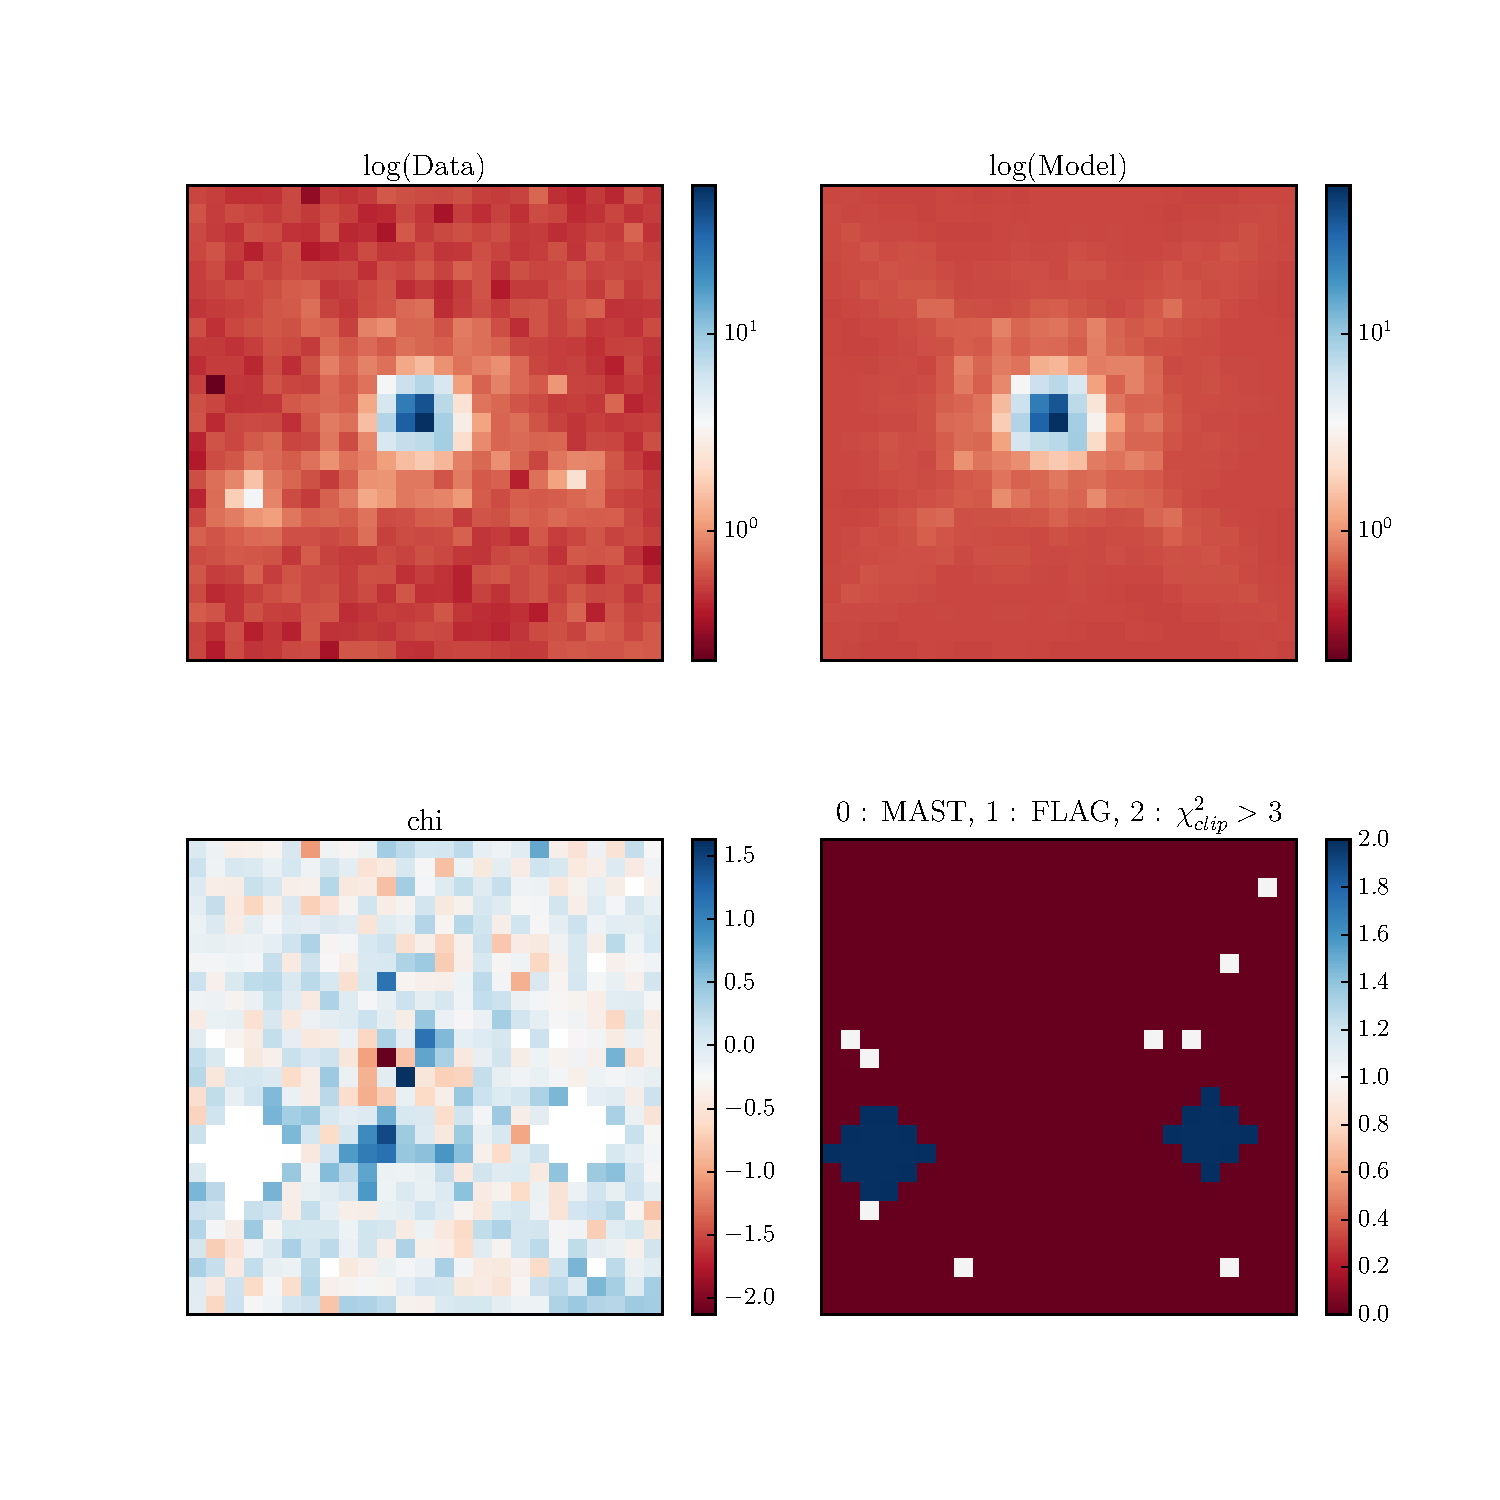
\includegraphics[width=0.9\textwidth]{figures/wfc3ir/example19.pdf}
\caption{\label{fig:validation_4} }
\end{figure*}


\begin{figure*}
%\begin{center}
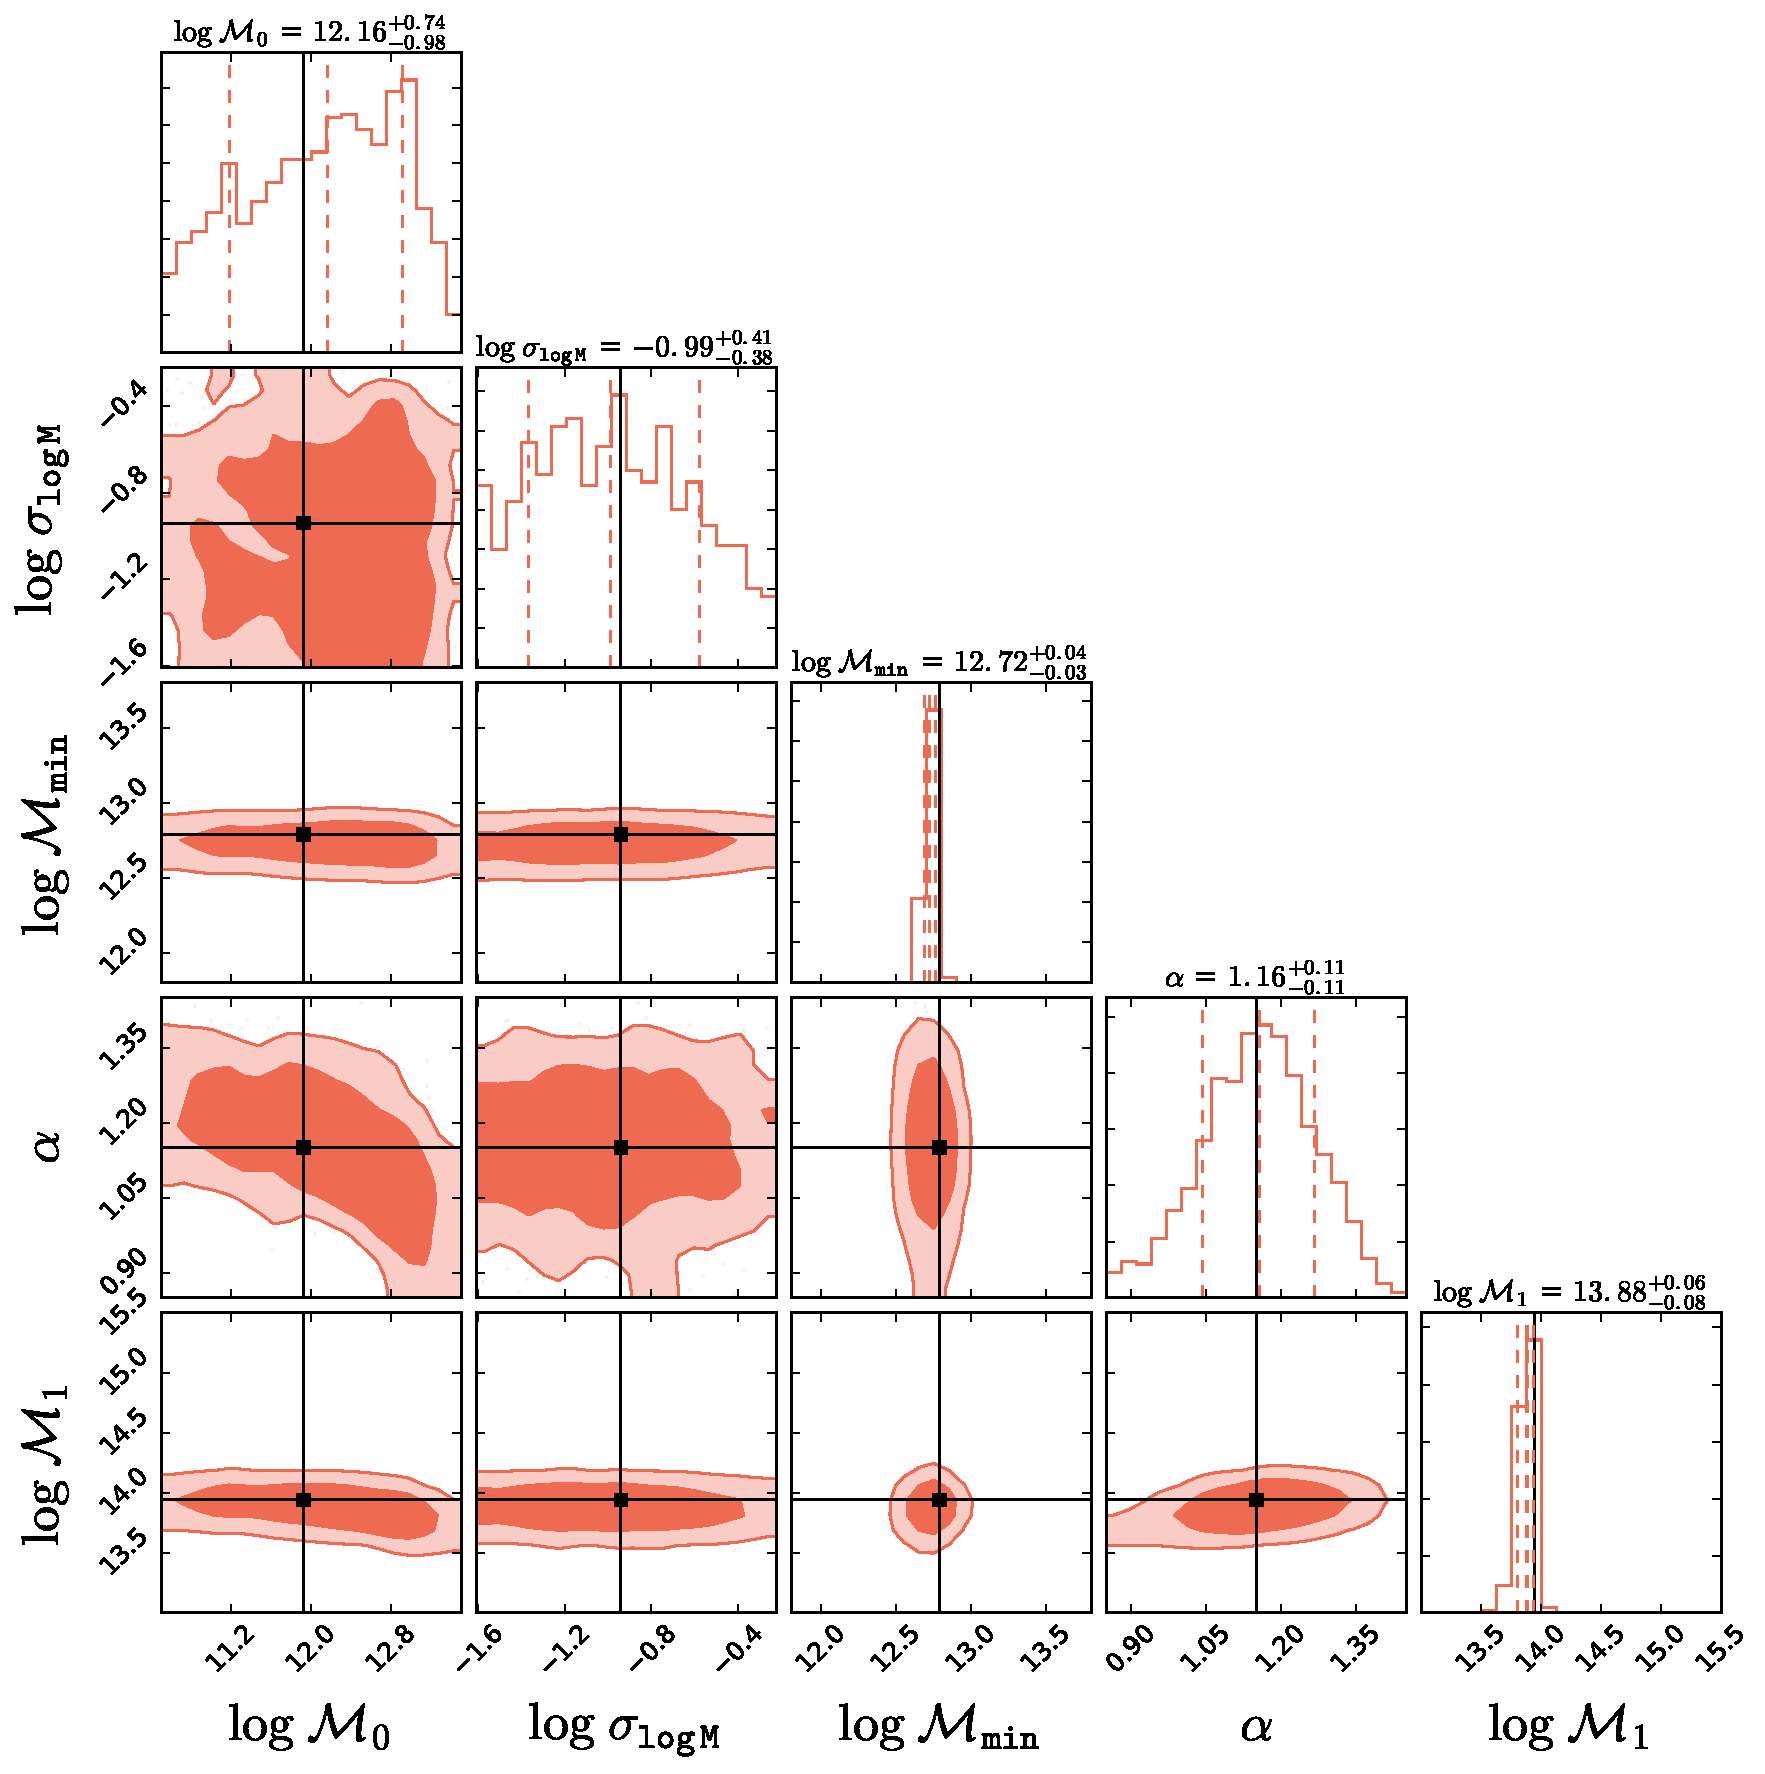
\includegraphics[width=0.85\textwidth]{figures/abc/paper_ABCcorner_nbarxi.pdf}
\caption{\label{fig:abc_corner_nbarxi} We present the constraints on the \citet{zheng07} HOD model parameters obtained from our ABC-PMC analysis using $\bar{n}$ and $\xigg(r)$ as observables.  
The diagonal panels plot the posterior distribution of each HOD parameter with 
vertical dashed lines marking the $50\%$ quantile and $68\%$ confidence intervals of the 
distribution. The off-diagonal panels plot the degeneracies between parameter pairs. 
The range of each panel corresponds to the range of our prior choice. The ``true''
HOD parameters, listed in Section \ref{sec:mock_obv}, are also plotted in each of 
the panels (black). For $\log\mathcal{M}_0$, $\alpha$, and $\sigma_{\log M}$, 
the ``true'' parameter values lie near the center of the $68\%$ confidence interval 
of the posterior distribution. For $\log\mathcal{M}_1$ and $\log\mathcal{M}_\mathrm{min}$, 
which have tight constraints, the ``true'' values lie within the $68\%$ confidence 
interval. Ultimately, the ABC parameter constraints we obtain in our analysis are consistent with the ``true'' HOD parameters.}
%\end{center}
\end{figure*}
